\section{Background}


	In diesem Kapitel sollen die verwenden Bibliotheken und der Grund für ihre Verwendung genauer beleuchtet werden. Damit wir Daten generieren konnten bzw. 
	können, haben wir die Bibliothek GetOldTweets3 verwendet. Mit einer öffentlich zugängliche Userliste für Politiker aus Amerika wurden dann mit diesem 
	Packages die Daten erhoben. Zur Weiterverarbeitung der Daten haben wir NLTK und TextBlob genutzt. Beides sind Tools für die Verarbeitung von Sprache. Um 
	eine Analyse über  die Verarbeiteten Ausgaben durch ein Map-Reduce laufen zu lassen, haben wir als letztes Package Sparks verwendet, um eine zeit 
	effiziente Verarbeitung zu gewährleisten.  
	
	 
	\subsection{GetOldTweets3-Pakage}
	
	GetOldTweets3 ist ein kostenlose Python 3 Packages mit welchen Twitterdaten ohne API-Schlüssel abgerufen werden können.
	Mit GetOldTweets3 können Sie Tweets mit einer Vielzahl von Suchparametern wie Start-/Enddatum, Benutzername(n), Textabfrage 
	und Referenzortbereich durchsuchen. Außerdem können Sie angeben, welche Tweet-Attribute Sie einbeziehen möchten. Einige Attribute
	sind: Nutzername, Tweettext, Datum, Retweets und Hashtags. \citeint{userguid} 
	Die offizielle API von Twitter hat eine lästige Zeiteinschränkung, weshalb man keine Tweets älter als eine Woche abrufen 
	kann. Es gibt einige Tools die Zugang zu älteren Tweets anbieten, diese sind jedoch meistens kostenpflichtig. Das Forscher-
	team hat nach einem andere Tool gesucht die diese Aufgaben übernehmen, wodurch die Wahl auf das Package GetOldTweets3 gefallen 
	ist. \citeint{python}   	
	Die Analyse des Codes von GetOldTweets3 und die Funktionsweise des Searchthrough Browsers von Twitter zeigt wie das Packages auch
	an alte Tweets kommt. Grundsätzlich, wenn sie auf Twitter seiten eingeben oder User suchen, startet ein Scroll-Loader. D.h. wenn sie
	dann weiter nach unten scrollen, bekommen sie immer mehr Tweets zu den Suchbegriffen. Diese ganzen Tweets bekommen sie durch Abfragen 
	an einen JSON-Provider. GetOldTweets3 imitiert den Searchthrough Browser von Twitter um den Scroll-Loader zu starten und zieht sich dann 
	anhand, der Abfragen an einen JSON-Provider die JSON-Datei und gibt diese decodiert zurück um dann alle Twitts anhand der oben gegebenen 
	Parameter herauszufiltern. Dies kann man in Quelle \citeint{github}, dem Github-Repositorium gut nachvollziehen. Somit ist es möglich sowohl 
	aktuelle als auch sehr alte Tweets zu scrapen. \citeint{github}
	
	
	\begin{figure}[ht]
		\centering
		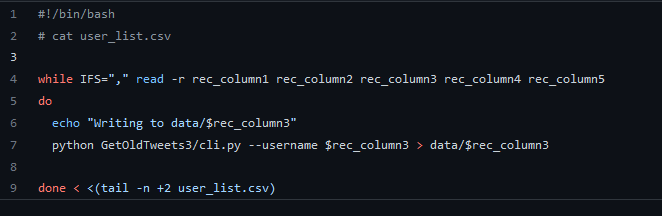
\includegraphics[width=0.9\textwidth]{images/Kapitel2/Code_Beispiel_1}
			\caption{\label{fig:CodeBeispiel}Code Beispiel für das Scrapen der Tweets}{Ist eine Python Bibliothek mit der Twitter Daten durch den Scroll-Loader 
			        des Searchthrough Browsers von Twitter als JSON-Datei abgerufen werden können.}
	\end{figure}
	
	So kann durch eine paar Zeilen Code, wie man in der Abbildung \label{CodeBeispiel} sieht, eine bash-Datei erstellt werden, durch welche die Daten gesucht 
	und abgespeichert werden. Das Scraping an sich kann durch die Größe der JSON-Datei einige Zeit in Anspruch nehmen. Wir haben gerade mal 2 Millionen Tweets 
	insgesamt bei einer Laufzeit von ca. 35 Stunden.  
	

	\subsection{NLTK-Natural language Toolkit}
	
	NLTK ist ein Python Package für die Arbeit mit menschlichen Sprachdaten. Es bietet einfach zu bedienende Schnittstellen zu über 50 Korpora
	und lexikalischen Ressourcen wie WordNet, zusammen mit einer Reihe von Textverarbeitungsbibliotheken für Klassifizierung, Tokenisierung, 
	Stemming, Tagging, Parsing und semantische Schlussfolgerungen, Wrapper für industrielle NLP-Bibliotheken und ein aktives Diskussionsforum. \citeint{nltk} 
	Aus diesem Grund bietet NLTK sehr viele Möglichkeiten zur Vorverarbeitung und Analyse, benötigt aber auch einen gewissen Zeitrahmen zur 
	Einarbeitung in die Analysen. Aus diesen Grund hat sich das Forscherteam dafür entschieden NLTK nur zur Vorverarbeitung zu nutzen und TextBlob
	für die Semantische Analyse zu nutzen. Warum sich für TextBlob entschieden wurde, wird genauer in 2.1.3 besprochen. So verwenden wir den Wordcorbus
	von NLTK für englische Stoppworte, da wir diese nicht mit in unseren Analysen haben wollen. Für eine individuelle und sehr ausführliche semantische Analyse 
	bietet NLTK sehr viele Möglichkeiten, durch die Interaktion mit verschiedenen Packages in Python, was aber den oben genannten Zeitrahmen benötigt, zum 
	einarbeiten. Der Vorteil von NLTK gegenüber TextBlob sind genau diese Interaktionen mit anderen Packages. Für größere Projekte, bei denen man die 
	semantische Analyse auch individuell anpassen möchte,sollte man eher die NLTK Bibliothek benutzen. NLTK ermöglicht es durch verschiedene 
	Vorverarbeitungsschritte, welche in der Bibliothek eingebaut sind eine individuelle Pipeline und Analyse zu erstellen.
	
	\begin{figure}[ht]
		\centering
		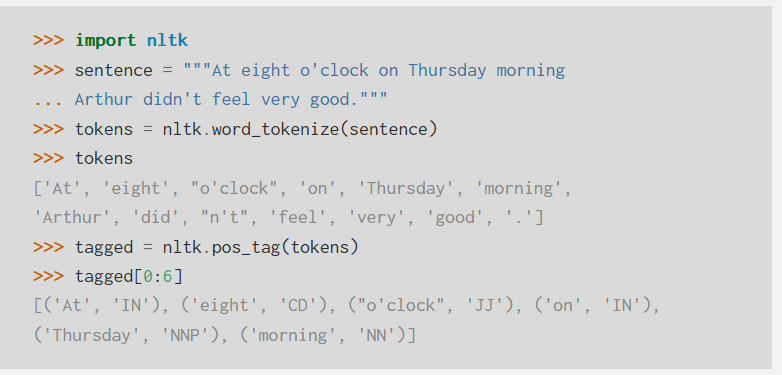
\includegraphics[width=0.9\textwidth]{images/Kapitel2/Code_Beispiel_2}
			\caption{\label{fig:CodeBeispiel}Code Beispiel für das Arbeiten mit NLTK}{Tokenizierung und Tagging von Texten mit NLTK}
	\end{figure}    	
		
	
	
	\subsection{TextBlob}
	
	TextBlob ist eine Python Bibliothek für Python zwei und drei. Diesem Package arbeiten, ähnlich wie NLTK, mit verschiedenen Packages welche in Python schon 
	verfügbar sind. In TextBlob sind zwei verschiedene Semantische Analysen vorhanden. Da gibt es zum einen die Patternanalyse verwendet, welche die Pattern 
	libary in Python von Python nutzt, und dann gibt es da noch die Naive-Bayes-Analyse. \citeint{blob} Hier stellt NLTK zum Beispiel mehr zur Verfügung, aber 
	benötigt damit auch mehr Einarbeitungszeit. Damit bietet TextBlob eine besser Übersicht, weshalb sich das Forscherteam auf Grund der wenigen Zeit für 
	diese Bibliothek entschieden hat. Ein weiter Grund, warum sich schlussendliche für diese Bibliothek entscheiden wurde, ist auch die zwei Outputwerte 
	Polarität und Subjektivität eine gute Anwendungsmöglichkeit für ein Mapreduce darstellen. \citeint{userguideText}	
	In unseren Analysen haben wir die Patternanalyse von TextBlob verwendet, welche uns die Polarität in einem Intervall von [-1, 1] und die Subjektivität im 
	Rahmen von [0, 1] zurück gibt. Ist der Wert bei der Polarität näher an der -1 als an der 1, dann zeigt es einen negative Emotion. Im umgekehrten Fall ist 
	es eine positive Emotion. Bei dem Wert der Subjektivität beschreibt ein Wert der näher an der Null ist eher einen Fakt oder Faktenwissen und je näher er 
	der 1 kommt, desto mehr spielt in die Aussage die eigene subjektive Meinung mit rein. \citeint{semtiment}\citeint{blobkgit}
	Bei der Patternanalyse geht es darum ein Muster bei negativen und positiven Aussagen zu erkennen und dies dann auf neue Testdaten oder unbekannte Daten 
	anzuwenden. Dabei spielt sowohl die Syntax als auch die Semantik und die Wortwahl eine große Rolle. \citeint{pattern}
	Mit etwas mehr Zeit hätte man auch noch die Analyse des Naive-Bayes in einem Mapreduce verwenden können.

	
	\subsection{Sparks}
	
	Sparks ist ein Big Data Framework zur Verarbeitung, Filterung und Analyse von großen Datenmengen. Diese Bibliothek vereinfacht die Anwendung eines 
	Mapreduce, indem es verschiedene Funktionsweisen und Tools dafür anbietet. So begrenzt sich der Programmcode auf die wesentlichen Funktionen eines 
	Mapreduce und verschafft dadurch eine gut Übersicht über den Code. Des weiteren stellt Sparks verschiedene Datenstrukturen zur Verfügung, um die Arbeit mit 
	großen Datenmengen zu erleichtern. Dazu gehört zum Beispiel das Resilient Distributed Datasets (RDD). Ein weiter Vorteil den Sparks bietet ist die hohe 
	Verarbeitungsgeschwindigkeit der Daten.
	Aus diesen Gründen hat sich das Forscherteam entschieden für das Mapreduce, welches in dem Forschungsprojekt Anwendung finden soll, diese Bibliothek zu 
	verwenden.     
	

	
